\section{Работа с файловыми диалогами}
\subsection{Условие задания}
Выполнить задание. Вариант: <<Создать таблицу Work. В другой файл вывести данные о рабочих, занимающих данную должность. (Вариант 14)>>.

Разработать приложение в соответствии со своим вариантом.

Приложение должно выполнять следующие действия:

\begin{enumerate}
\item Заголовок формы должен отражать суть задания.
\item Все элементы формы должны быть внятно подписаны (кнопки подписаны, у тестового поля должно быть написано, для чего оно нужно и т.д.)
\item Структура представляет собой таблицу DataGridView, в ячейках которой записаны данные разных типов.
\item Предусмотреть кнопки:
\begin{itemize}
    \item считывание данных из файла и запись данных в таблицу (предполагается, что в файле данные корректные);
    \item возможность добавлять и удалять строки в таблице, соответственно, вводить данные вручную.
    \item запись в файл всех данных. Проверять корректность ввода данных: даты должны быть реальные, номер телефона состоять из цифр и, может быть, знак тире, оценки студентов - от 2 до 5. Все остальное можно не проверять. Если есть срок пребывания, дата прибытия и дата отбытия, то срок пребывания должен быть равен разнице между датой отбытия и датой прибытия.
    \item запись в файл данных по определенному критерию. Критерий можно вводить вручную через TextBox или выбирать c помощью Radiobox и т. д. Запись в файл должна быть такой, чтобы этот файл можно было открыть в приложении.
    \item запись данных по определенному критерию в новую таблицу. При выборе другого критерия старая таблица должна удаляться.
\end{itemize}
\item При неправильном вводе каких-либо данных таблица выбранных данных должна очищаться.
\item В коде должны быть комментарии и отступы (код должен быть легко читаем).
\end{enumerate}

\subsection{Вид формы в конструкторе}
Форма имеет вид как на рисунке \ref{fig:file-dialogs-form}

\begin{figure}
\centering
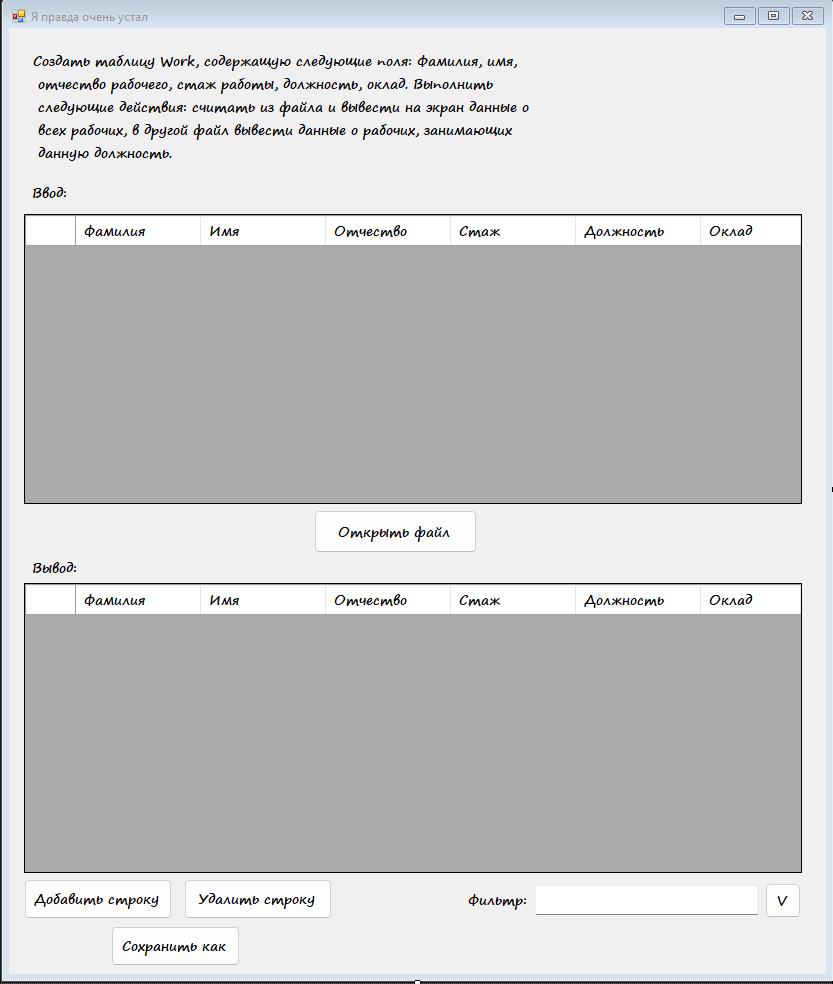
\includegraphics[width=0.5\linewidth]{images/file-dialogs/form.png}
\caption{Форма окна для задания}
\label{fig:file-dialogs-form}
\end{figure}

\subsection{Таблица с описанием элементов формы}
Все элементы формы были переименованы для большей читаемости. В таблице \ref{tab:file-dialogs-form} представлены все изменения.


\begin{xltabular}{\textwidth}{| m{0.3\textwidth} | m{0.3\textwidth} | m{0.3\textwidth} |}

\hline
\textbf{Описание элементов формы} & \textbf{Список изменённых атрибутов} & \textbf{Новое значение атрибута} \\
\hline
\endfirsthead

\hline
\textbf{Описание элементов формы} & \textbf{Список изменённых атрибутов} & \textbf{Новое значение атрибута} \\
\hline
\endhead

\hline
\endfoot

\hline
\caption{Значение атрибутов элементов в приложении для работы с коллекциями}
\label{tab:file-dialogs-form}
\endlastfoot

Окно формы & Text & Я правда очень устал \\

Метка для задания & Name & labelTask \\
Метка <<Ввод>> & Name & lblInput \\
Метка <<Вывод>> & Name & lblOutput \\
Метка <<Фильтр>> & Name & labelFilter \\

Таблица для ввода & Name & dataGridInput \\
Таблица для вывода & Name & dataGridOutput \\

Кнопка <<Добавить строку>> & Name & btnAddRow \\
Кнопка <<Добавить строку>> & Name & btnRemoveRow \\
Кнопка <<Добавить строку>> & Name & btnSaveInFile \\
Кнопка <<Добавить строку>> & Name & btnReadFile \\
Кнопка <<Применить фильтр>> & Name & filterButton \\

Поле для ввода фильтра & Name & filterTextbox \\
\end{xltabular}


\subsection{Примеры правильной и неправильной работы приложения}
При запуске приложения на экране появляется окно \ref{fig:file-dialogs-start}.

\begin{figure}
\centering
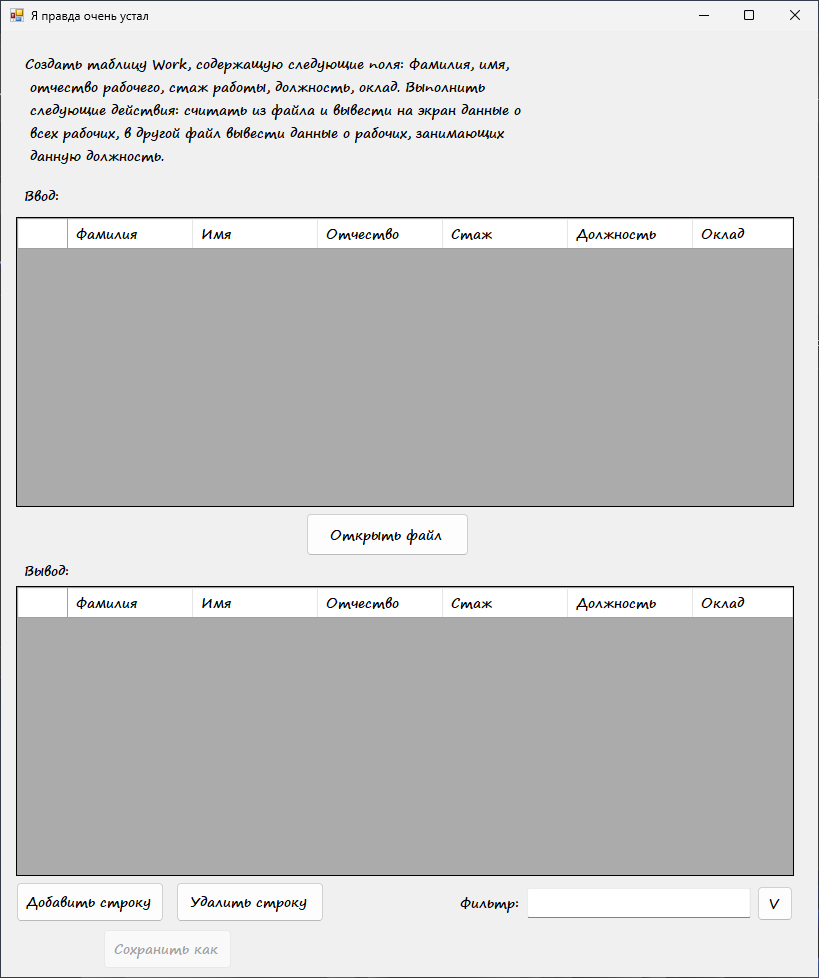
\includegraphics[width=0.5\linewidth]{images//file-dialogs/start.png}
\caption{Запуск программы}
\label{fig:file-dialogs-start}
\end{figure}

При нажатии на кнопку всё обрабатывается корректно. Также происходит обработка ошибок.

\begin{figure}
\centering
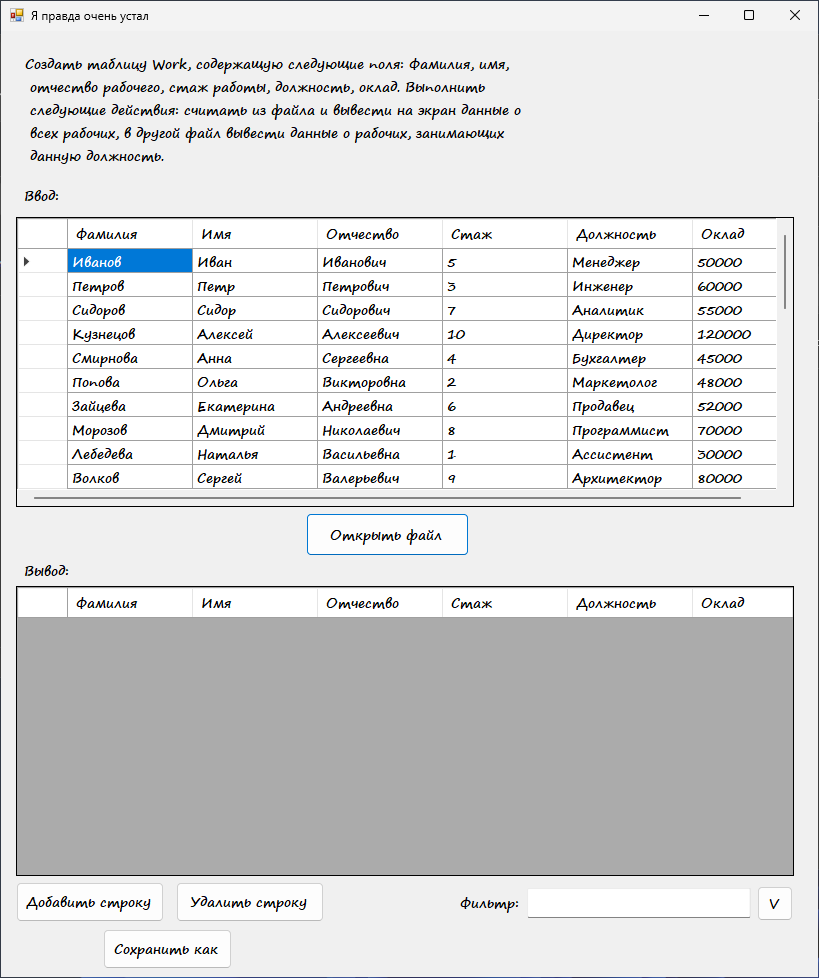
\includegraphics[width=0.5\linewidth]{images//file-dialogs/okay.png}
\caption{Запуск с корректными данными}
\label{fig:file-dialogs-okay}
\end{figure}

\begin{figure}
\centering
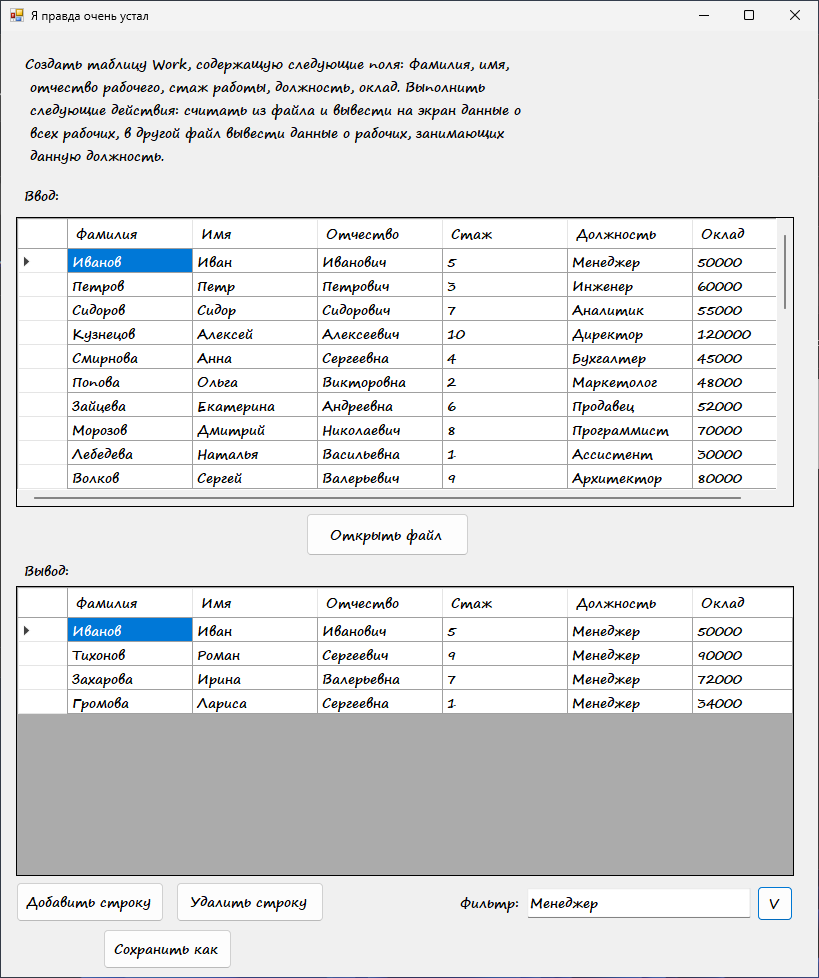
\includegraphics[width=0.5\linewidth]{images//file-dialogs/okay1.png}
\caption{Запуск с корректными данными}
\label{fig:file-dialogs-okay}
\end{figure}

\begin{figure}
\centering
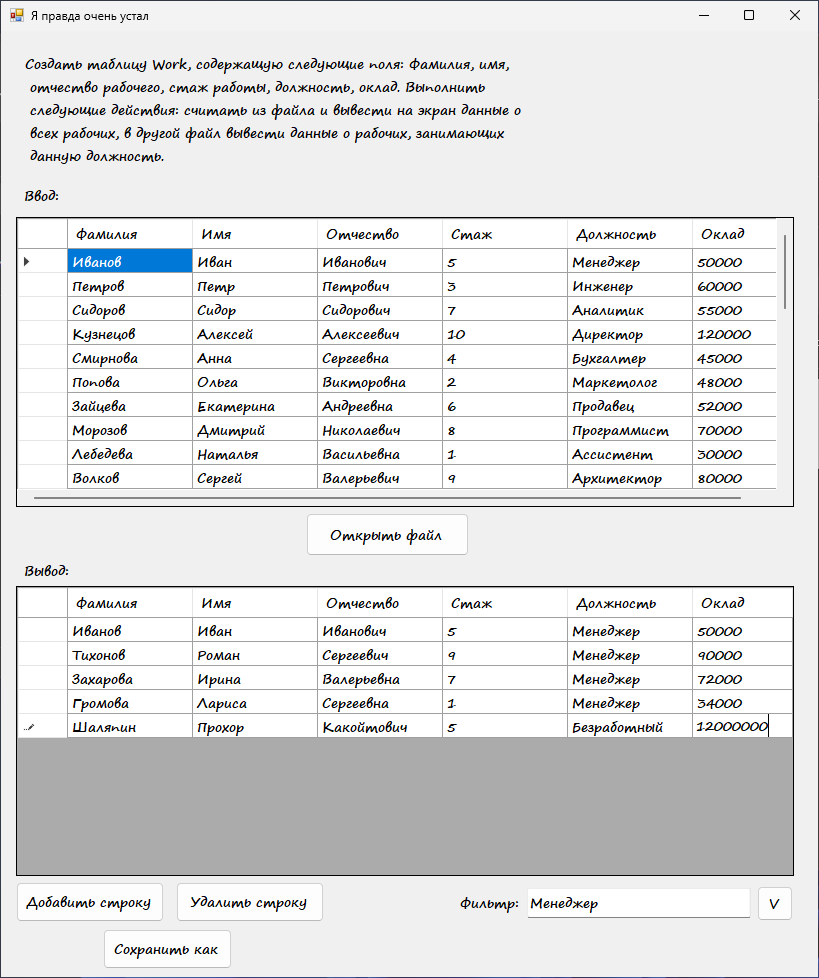
\includegraphics[width=0.5\linewidth]{images//file-dialogs/okay2.png}
\caption{Запуск с корректными данными}
\label{fig:file-dialogs-okay}
\end{figure}

\begin{figure}
\centering
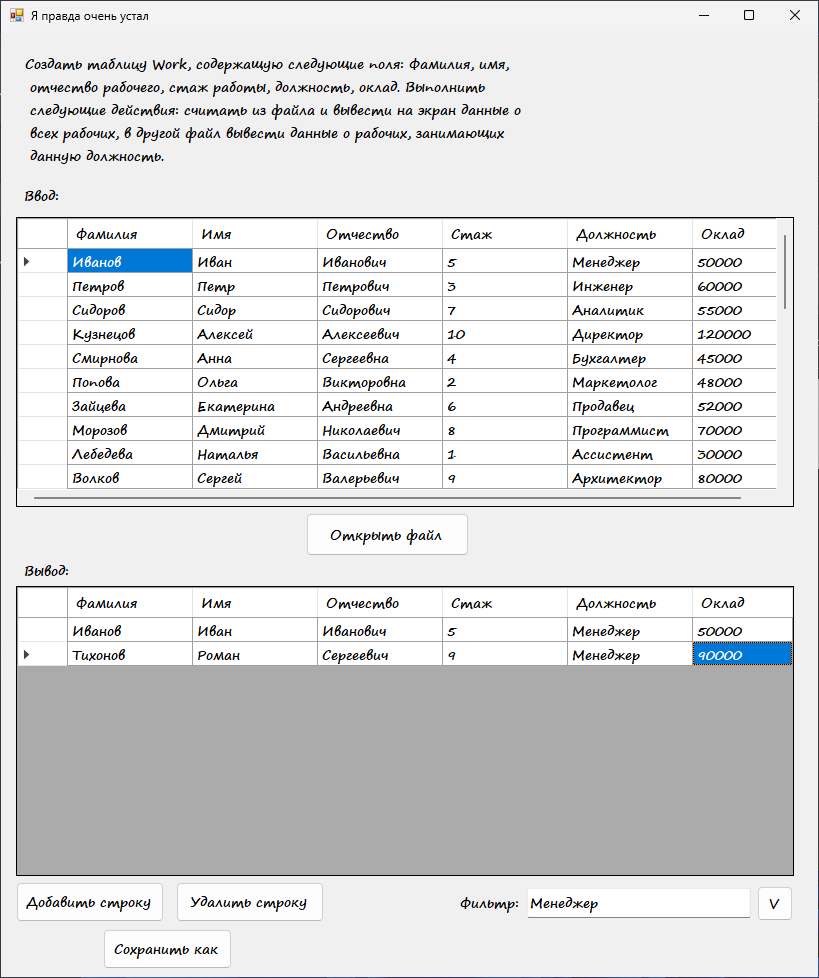
\includegraphics[width=0.5\linewidth]{images//file-dialogs/okay3.png}
\caption{Запуск с корректными данными}
\label{fig:file-dialogs-okay}
\end{figure}

\begin{figure}
\centering
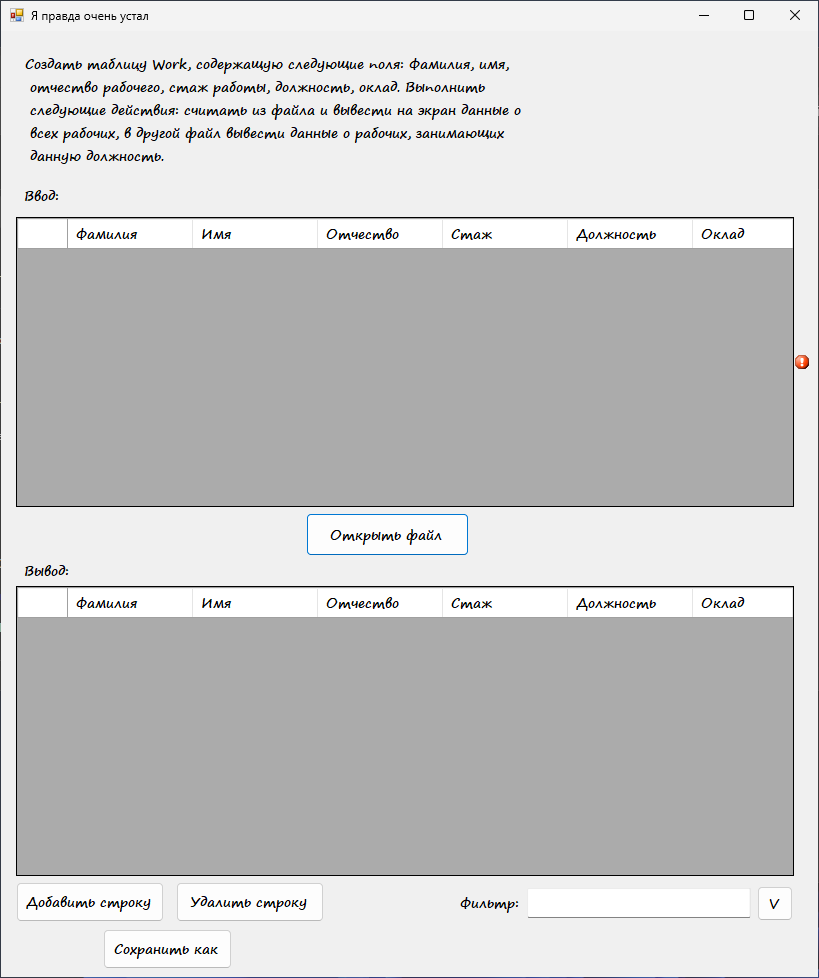
\includegraphics[width=0.5\linewidth]{images//file-dialogs/error.png}
\caption{Пример ввода с некорректными данными}
\label{fig:file-dialogs-error}
\end{figure}

\begin{figure}
\centering
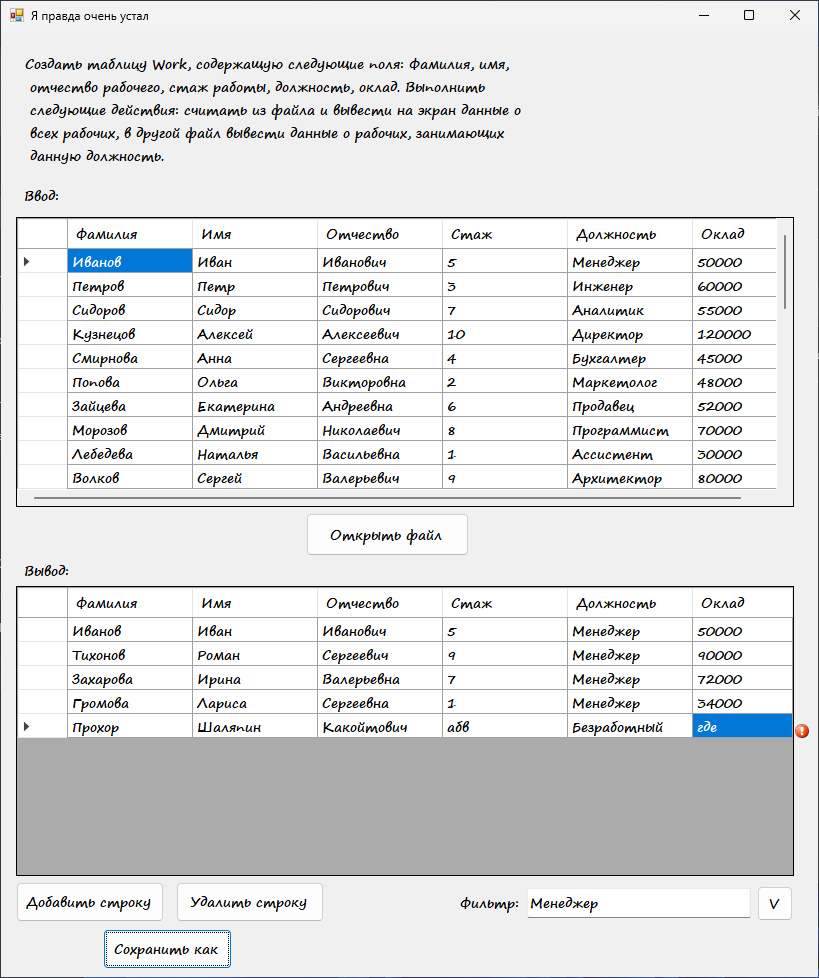
\includegraphics[width=0.5\linewidth]{images//file-dialogs/error2.png}
\caption{Пример ввода с некорректными данными}
\label{fig:file-dialogs-error2}
\end{figure}


\subsection{Примеры исходного кода}
\begin{minted}{cpp}
private: System::Void filterButton_Click(System::Object^ sender, System::EventArgs^ e) {
this->dGrOutput->Rows->Clear();
for (int i = 0; i < this->dGrInput->RowCount; ++i) {
    if (this->dGrInput->Rows[i]->Cells[4]->Value->Equals(filterTextbox->Text)) {
        this->dGrOutput->Rows->Add(this->dGrInput->Rows[i]->Cells[0]->Value,
                                this->dataGridInput->Rows[i]->Cells[1]->Value,
                                this->dataGridInput->Rows[i]->Cells[2]->Value,
                                this->dataGridInput->Rows[i]->Cells[3]->Value,
                                this->dataGridInput->Rows[i]->Cells[4]->Value,
                                this->dataGridInput->Rows[i]->Cells[5]->Value);
    }
}
}
\end{minted}

Больше кода проекта доступно в приложении \ref{application-A}. Также в приложенном архиве можно найти полный код проекта.